\documentclass{article}

% Some useful packages.
\usepackage{amsmath}
\usepackage{siunitx}
\usepackage{graphicx}
\usepackage{verbatim}
\usepackage{mhchem}
\usepackage{textcomp}
\usepackage{courier}
\usepackage{listings}

% Reduces margins substantially.
\usepackage{geometry}
\newgeometry{margin=2.5cm}

% Allows headers and footers.
\usepackage{fancyhdr}
\pagestyle{fancy}
% Get rid of annoying line under header.
\renewcommand{\headrulewidth}{0pt}

\lhead{}
\chead{}
\rhead{}

\lstset{
    basicstyle=\ttfamily,
}

% Answers concise.
% Don't reproduce analysis from notes, just refer to results.

\begin{document}

\section*{MTMW14 Project 2: Using Shallow Water Equations to Model Ocean Gyres}

\section*{SN: 23865130}

\section*{Introduction}

In this project a model of a large scale ocean gyre is developed. The model is based on the Shallow
Water Equations (SWEs), linearised about a resting state:

\begin{align}
    \label{eqn:swe1} 
    \frac{\partial \eta}{\partial t} & =  - H (\frac{\partial u}{\partial x} + \frac{\partial v}{\partial y} ),  \\
    \label{eqn:swe2} 
    \frac{\partial u}{\partial t} & =  + (f_0 + \beta y) v - g \frac{\partial \eta}{\partial x} - \gamma u + \frac{\tau_x}{\rho H}, \\
    \label{eqn:swe3} 
    \frac{\partial v}{\partial t} & =  - (f_0 + \beta y) u - g \frac{\partial \eta}{\partial y} - \gamma v + \frac{\tau_y}{\rho H}.
\end{align}

Here $\eta$ represents the height perturbation, $u$ and $v$ represent the column averaged zonal and meridional
velocity perturbations. $H$ is the average height, $f_0$ and $\beta$ are the Coriolis and $\beta$
parameters, $g$ is the acceleration due to gravity, $gamma$ represents drag processes, and $\tau_x$
and $\tau_y$ represent the wind stress forcings. The equations were solved using a square domain,
with the sides being given by $L$.  The values used for the parameters were: 


\begin{center}
    \begin{tabular}{ c|r l } 
	parameter & value & unit \\ 
	\hline
	$L$ & \SI{1e6}{} & \SI{}{m} \\
	$H$ & \SI{1000}{} & \SI{}{m} \\ 
	$f_0$ & \SI{1e-4}{} & \SI{}{s^{-1}} \\ 
	$\beta$ & \SI{1e-11}{} & \SI{}{m^{-1} s^{-1}} \\ 
	$g$ & \SI{10}{} & \SI{}{m s^{-2}} \\ 
	$\gamma$ & \SI{1e-6}{} & \SI{}{s^{-1}} \\ 
	$\rho$ & \SI{1000}{} & \SI{}{kg m^{-3}} \\ 
	$\tau_x$ & $-cos(\frac{\pi y}{L})$ & XX \\ 
	$\tau_y$ & 0 & XX \\ 
    \end{tabular}
\end{center}


Following (XX Matsuno Beckers Deleersnijder) the SWEs are solved on an Arakawa-C grid using the
forward-backward time scheme. The Arakawa-C grid was chosen so that e.g. spatial derivatives of $u$
in the $x$ direction would be available at the points where $\eta$ is calculated. The domain is
taken to be the size of the $\eta$ grid points, as can be seen in Figure \ref{fig:arakawa_c_grid}.
First $\eta$, $u$ then $v$ are calculated:

\begin{align}
    \label{eqn:swe_arakawa1} 
    \eta^{n+1} & =  \eta^n- H \Delta t (\frac{\partial u^n}{\partial x} + \frac{\partial v^n}{\partial y} ),  \\
    \label{eqn:swe_arakawa2} 
    u^{n+1} & = u^n + (f_0 + \beta y) \Delta t v^n - g \Delta t \frac{\partial \eta^{n+1}}{\partial
    x} - \gamma \Delta t u^n + \Delta t \frac{\tau_x}{\rho H}, \\
    \label{eqn:swe_arakawa3} 
    v^{n+1} & = v^n - (f_0 + \beta y) \Delta t u^{n+1} - g \Delta t \frac{\partial \eta^{n+1}}{\partial y} -
    \gamma \Delta t v^n + \Delta t \frac{\tau_y}{\rho H}.
\end{align}

Second $\eta$, $v$ then $u$ are calculated:

\begin{align}
    \label{eqn:swe_arakawa4} 
    \eta^{n+2} & =  \eta^{n+1}- H \Delta t (\frac{\partial u^{n+1}}{\partial x} + \frac{\partial
    v^{n+1}}{\partial y} ),  \\
    \label{eqn:swe_arakawa5} 
    v^{n+2} & = v^{n+1} - (f_0 + \beta y) \Delta t u^{n+1} - g \Delta t \frac{\partial \eta^{n+2}}{\partial y} -
    \gamma \Delta t v^{n+1} + \Delta t \frac{\tau_y}{\rho H}, \\
    \label{eqn:swe_arakawa6} 
    u^{n+2} & = u^{n+1} + (f_0 + \beta y) \Delta t v^{n+2} - g \Delta t \frac{\partial
	\eta^{n+1}}{\partial x} - \gamma \Delta t u^{n+1} + \Delta t \frac{\tau_x}{\rho H}.
\end{align}

% Say something about Rossby radius of deformation and link to spatial resolution.
% Justify timestep/etc.


\section*{Task A}

\begin{figure}[ht!]
    \centering
    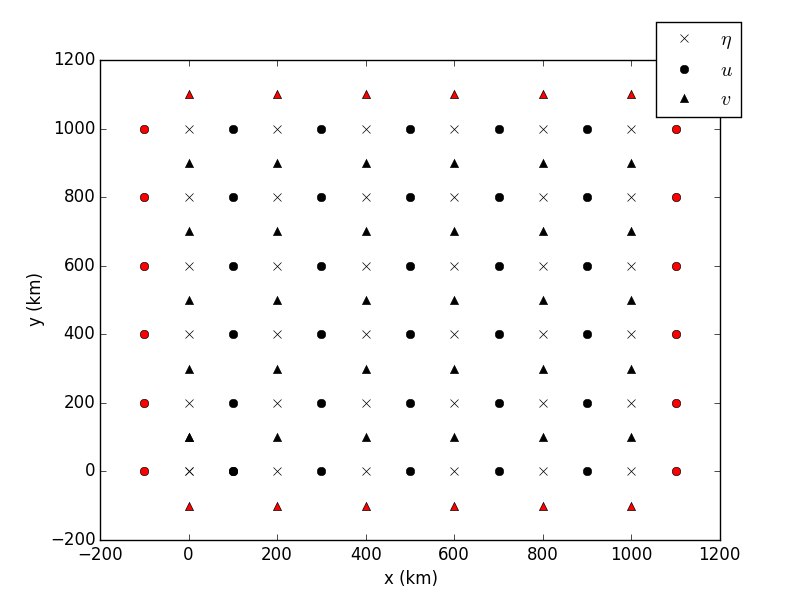
\includegraphics[width=300px]{figures/arakawa_c_grid}
    \caption{Shows where $\eta$, $u$ and $v$ are calculated on the Arakawa-C grid for $\Delta x =
	\Delta y = 250000  m$ (lower than the lowest resolution used in this project, for
	illustration only). Note, $u$ is one bigger in the $x$ direction than $\eta$ (and similar
	for $v$ in $y$ direction), and therefore the minimum and maximum $u$ coordinates lie
	$\frac{\Delta x}{2}$ outside the domain (and similar for $v$). The red grid-point values
	show values which are held at $0$ due to the boundary conditions. }
    \label{fig:arakawa_c_grid}
\end{figure}


\subsection*{Dispersive nature of CTCS}

The shortwave oscillations in the CTCS solutions, as seen by oscillations to the left of the largest
changes in gradient, are caused by the dispersive nature of CTCS. This can be explained by the
dispersion relationship for CTCS. This dispersion relationship is derived by considering what
happens to the amplification factor for CTCS, and can be used to show that the numerical phase
velocity of the waves is given by:

\begin{equation}
    \sin \alpha = c \sin k \Delta x
\end{equation}

\begin{equation}
    \frac{u_n}{u} = \pm \frac{\alpha}{c k \Delta x}\\
\end{equation}


\section*{Appendix A}

All code can be downloaded from the following link:

https://github.com/markmuetz/mtmw14

\end{document}

\end{document}
